\documentclass[twoside,twocolumn]{article}

\usepackage{blindtext} 
\usepackage{graphicx}
\usepackage[sc]{mathpazo} 
\usepackage[T1]{fontenc} 
\linespread{1.05} 
\usepackage{microtype} 


\usepackage[english]{babel} 


\usepackage[hmarginratio=1:1,top=32mm,columnsep=20pt]{geometry} 
\usepackage[hang, small,labelfont=bf,up,textfont=it,up]{caption} 
\usepackage{booktabs} 


\usepackage{lettrine} 


\usepackage{enumitem} 
\setlist[itemize]{noitemsep} 


\usepackage{abstract} 
\renewcommand{\abstractnamefont}{\normalfont\bfseries} 
\renewcommand{\abstracttextfont}{\normalfont\small\itshape} 


\usepackage{titlesec} 
\renewcommand\thesection{\Roman{section}} % 
\renewcommand\thesubsection{\roman{subsection}} 
\titleformat{\section}[block]{\large\scshape\centering}{\thesection.}{1em}{} 
\titleformat{\subsection}[block]{\large}{\thesubsection.}{1em}{} 


\usepackage{fancyhdr} 
\pagestyle{fancy} 
\fancyhead{} 
\fancyfoot{} 
\fancyhead[C]{ Unidad I : Articulo del Proyecto ICC-OJU-PJ $\bullet$ Septiembre 2020 $\bullet$ } 
\fancyfoot[RO,LE]{\thepage} 


\usepackage{titling} 


\usepackage{hyperref} 


%----------------------------------------------------------------------------------------
%	TILULOS
%----------------------------------------------------------------------------------------


\setlength{\droptitle}{-4\baselineskip} 

\pretitle{\begin{center}\Huge\bfseries} 
\posttitle{\end{center}} 
\title{Implementación de Call Center y Orientación Jurídica Al Usuario para el Poder Judicial} 
\author{Samuel Nuñez Mamani - Franklin Carlos, Huichi Contreras, \\
Anthony Robles Flores. }
\date{\today} 
\renewcommand{\maketitlehookd}{
\begin{abstract}
\noindent 
Determino las estrategias que debiera tenerse en cuenta para planificar, estructurar y finalmente escribir un articulo o “paper” de Ciencias Sociales
conforme a la Asociacion Americana de Psicologa (APA) Sexta Edicion. Se pretende que el lector produzca su propio trabajo.
\end{abstract}
\begin{abstract}
\noindent 

Treva es un sistema enfocado en los formularios de satisfacion del cliente en donde el propietario podra generar formularios y enviar cada cierto tiempo a sus empleado o interesados para que puedan llenarlo segun
las opciones que cuenta el formulario, a partir de esos datos podemos al propietario dar estadisticas en la cual puede verificar que opciones escogieron los clientes o empleados, y aparte de ello podemos analizar los datos
para dar recomendaciones o proyecciones estimadas de areas especificas.

\end{abstract}
}

%----------------------------------------------------------------------------------------

\begin{document}

% Print the title
\maketitle

%----------------------------------------------------------------------------------------
%	INTRODUCCION
%----------------------------------------------------------------------------------------

\section{Introduccion}
\lettrine[nindent=0em,lines=3]{A}ctualmente en el Perú las pequeñas y medianas empresas producen al mercado peruano ingresos y empleo, la gran cantidad de informacion que manejan es debido al alto numero de operaciones que realizan a diario, por lo tanto se necesita una forma de controlar los datos como las opiniones de los clientes y de esta forma conseguir retroalimentacion instantanea para las empresas. Asimismo tener la informacion en reportes descriptivos para la visualizacion se ha hecho parte importante de los sistemas de hoy para tomar desiciones acertadas y utiles para las empresasl.

\section{Titulo}
El sistema se identifica con el titulo de treva.

\section{Autores}
\begin{itemize}
\item Anthony Richard , Robles Flores.
\item Franklin Carlos, Huichi Contreras.
\item Samuel, Nuñez Mamani.
\end{itemize}

\section{Planteamiento del problema}
\subsection{Problema}
La problematica general es el como las empresas evaluan el desempeño de sus servicios, y como pueden medir la satisfacción del cliente al igual de saber la efectividad y el buen manejo de sus productos.

\subsection{Justificacion}
Hoy en día los datos toman cada vez mas valor en una organizacion o empresa, de esta manera pueden asegurar una ventaja contra sus competidores y así beneficiarce para obtener una mejor calidad de servicio, mejorar su producto y por consiguiente clientes satisfechos.

\subsection{Alcance}
Para el alcance de este proyecto nesecitaremos de clientes que quieran realizar sus formularios de satisfaccion y ofrecerles todas las herramientas nesecarias para que lo hagan de manera eficaz. Alcanzado la meta podremos generar los dashboards que ayude al cliente a ver los resultados entre otros indicadores.


\section{Objetivos}
\subsection{General}
Determinar el nivel de satisfaccion de los clientes de las empresas afiliadas a treva

\subsection{Especificos}
\begin{itemize}
\item Mejorar el rendimiento de las empresas con reportes estadisticos en las encuestas realizadas sobre el nivel de satisfaccion de los clientes, que se usaran para la toma de desiciones.
\item Comparar los grados de satisfacción de los clientes periodicamente.
\item Definir la relación real entre encuestas y satisfacción del cliente.
\end{itemize}

\section{Referentes teoricos}
La idea nos nacio como grupo luego de ver ejemplos de paginas como bimatico en donde manejaban estadisticas de la realizacion de las estadisticas de cada pregunta y area realizada
a continuacion pondre un ejemplos realizados esta pagina. Apartir de esas estadisticas nos dimos cuenta que pdoriamos realizar un sistema que pueda controlar todo esto desde el punto inicial hasta llegar al punto de los reportes.


\section{Descripcíon del Proyecto}
\subsection{Problemática}
Actualmente a nivel Mundial la aparición del Covid19 a provocado un desorden Global, para que este virus no se propague, nuestro Gobierno fue obligado a decretar un "Estado de Emergencia" a nivel nacional provocando asi una paralización brusca en la gran mayoría de trabajos.
\\
Esto provocó un adaptamiento brusco a continuar con las jornadas laborales pero de forma virtual , utilizando asi todos los canales de comunicación posibles.
El personal de muchas organizaciones pasaron de sus jornadas agregando un plus extra el cual es estar pendiente en todos los canales de comunicación para el usuario.
\\
El Poder Judicial de Tacna, atraviesa esta situación provocando que las jornadas sean prescenciales y virtuales, sumandole a esto una saturación constante de llamadas para  interrogantes existentes por parte del usuario provocando asi un retraso en sus actividades cotidianas y también una molestia constante por la gran cantidad de llamadas entrantes a su respectivo anexo como resultado llevarlos a un cuadro de estrés que en un futuro podría perjudicarles en su labores.

\subsection{Propuesta de Solución}
Para solucionar esta problemática existente en el poder judicial tomando en cuenta estos tiempos de la pandemia donde el asilamiento social a provocado un desbalance en las actividades normales de los trabajadores en esta entidad sobrecargando con labores adicionales para el proceso de adaptamiento a este contexto en el que vivimos , la implementacion de un Call Center podría agilizar los procesos de los trabajadores donde un asistente podria solucionar las interrogantes que podrian tener los usuarios antes que un trabajador interno pueda intervenir, pero en caso el asistente no pudiese resolver esta duda , el mismo call center podria derivar a un anexo a poder comunicarse vía telefonica con un asesor legal.
\\
Viendo que existen diferentes canales de comunicación,  en el momento de interactuar con el usuario , proponemos tambien una aplicacion Móvil en Android donde este prodrá otorgar los mismos servicios añadiendo tambien la facilidad al usuario de poder ubicar las oficinas de acuerdo a la sucursal en la que necesiter asistir a una cita programada , como tambien  el llenado de formularios con formatos ya establecidos por el poder judicial donde hay algunos documetos que no se necesiten la evaluacion de un abogado y como resultado la aplicacion podría descargar un PDF con los datos solicitados usando el formato de documentos del Poder Judicial.
\\
Tomando en cuenta que la tecnologia de tener un SmartPhone invade cada vez mas a la sociedad , incluir un módulo en el aplicativo acerca de las audiencias que el poder judicial publicará asi el usuario externo podría tener a la mano esta información a fin de poder asistir y estar pendientes puesto que en la web se encuentra el cronograma pero ubicar una audiencia para aquellos que desconocen el uso de una plataforma web podria ser dificultoso , la aplicacion movil podria ayudar a que sera mas sencillo y rápido de identificar una audiencia.

\subsection{Tecnologíaa de información}
En esta seccion definiremos las herramientas que se utilizaran para el desarrollo del proyecto asi mismos las plataformas que se emplearan para las conexiones en algunos servicios.
\begin{itemize}
\item Plataforma Colaborativa
\subitem Github : Una herramienta colaborativa muy útil en el control de versiones para el desarrollo de un Proyecto de Software con la capacidad de poder crear ramas para el crecimiento en escala de menor a mayor de un Sistema.
\subitem Google Meet : Una aplicación de videoconferencia que permitirá a los integrantes de grupo poder entablar una comunicación virtual para poder facilitar el trabajo en equipo.
\subitem Teams Microsoft : Plan de contigencia en caso el Google meet pueda caer, puede ser usado puesto que la propia Universidad Privada de Tacna puede otorgar a los estudiantes para realizar videconferencias interactivas con los integrantes del grupo de proyecto con múltiples herramientas que ayudarán para la colaboracion en la elaboración de este proyecto.
\item Base de Datos:
\subitem Firebase RealTime DataBase : Nos permitirá sincronizar datos con nuestra Base de Datos NoSQL alojada en la nube, estos datos se sincronizaran con todos los clientes en tiempo real.
\item Lenguajes de programación:
\subitem Lenguaje Java.
\item Entorno de Desarrollo:
\subitem Android Studio : Entorno que nos permitirá desarrollar aplicaciones móviles.
\item Asistente Virtual:
\subitem DialogFlow : Plataforma que nos permitirá agentes virtuales o asistentes virtuales para una futura integración en multiples canales de comunicación.
\item Red Telefonica:
\subitem VoximPlant.
\end{itemize}

\subsection{Arquitectura del Call Center}

\begin{figure}[h!]
	\begin{center}
		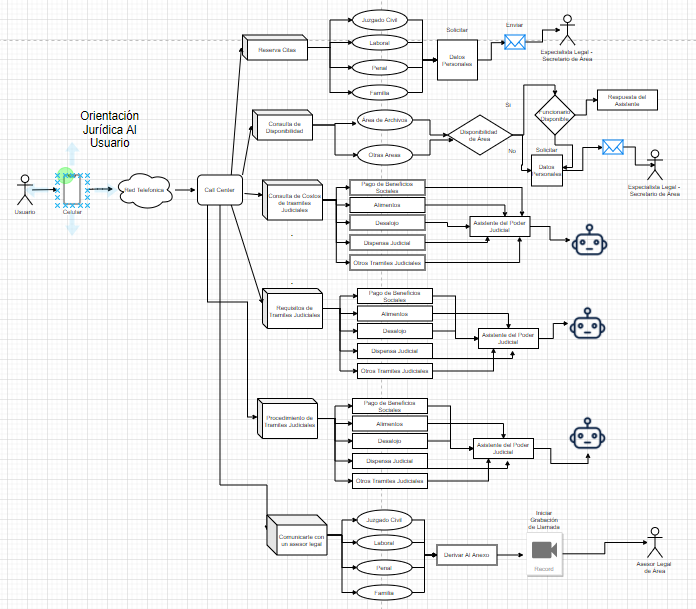
\includegraphics[width=7.5cm]{./Imagenes/callcenter} 
		\caption{Call Center}
	\end{center}
\end{figure}


\subsection{Metodología}
La metodologia que usaremos será RUP (Proceso Unificado de Rational)puesto que esta metodología provee un entorno de desarrollo flexible basado en estándares que se adapta a las necesidades del desarrollador o de las empresas y tener la facilidad de dividir todas las actividades de forma de que a cada participantele pueda tocar la parte que le compete.

\subsection{Arquitectura de la Aplicación}

\begin{figure}[h!]
	\begin{center}
		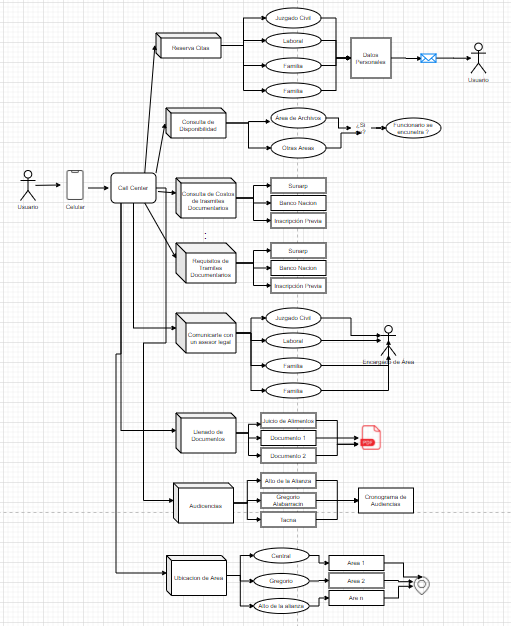
\includegraphics[width=7.5cm]{./Imagenes/apk} 
		\caption{Aplicación Movil}
	\end{center}
\end{figure}

\section{Conclusiones}

\end{document}
